\section{Appendix}

  \subsection{Appendix A - Partnerships Objectives}
    \label{sec:AppendixA}
    \begin{figure}[H]
      \centering
      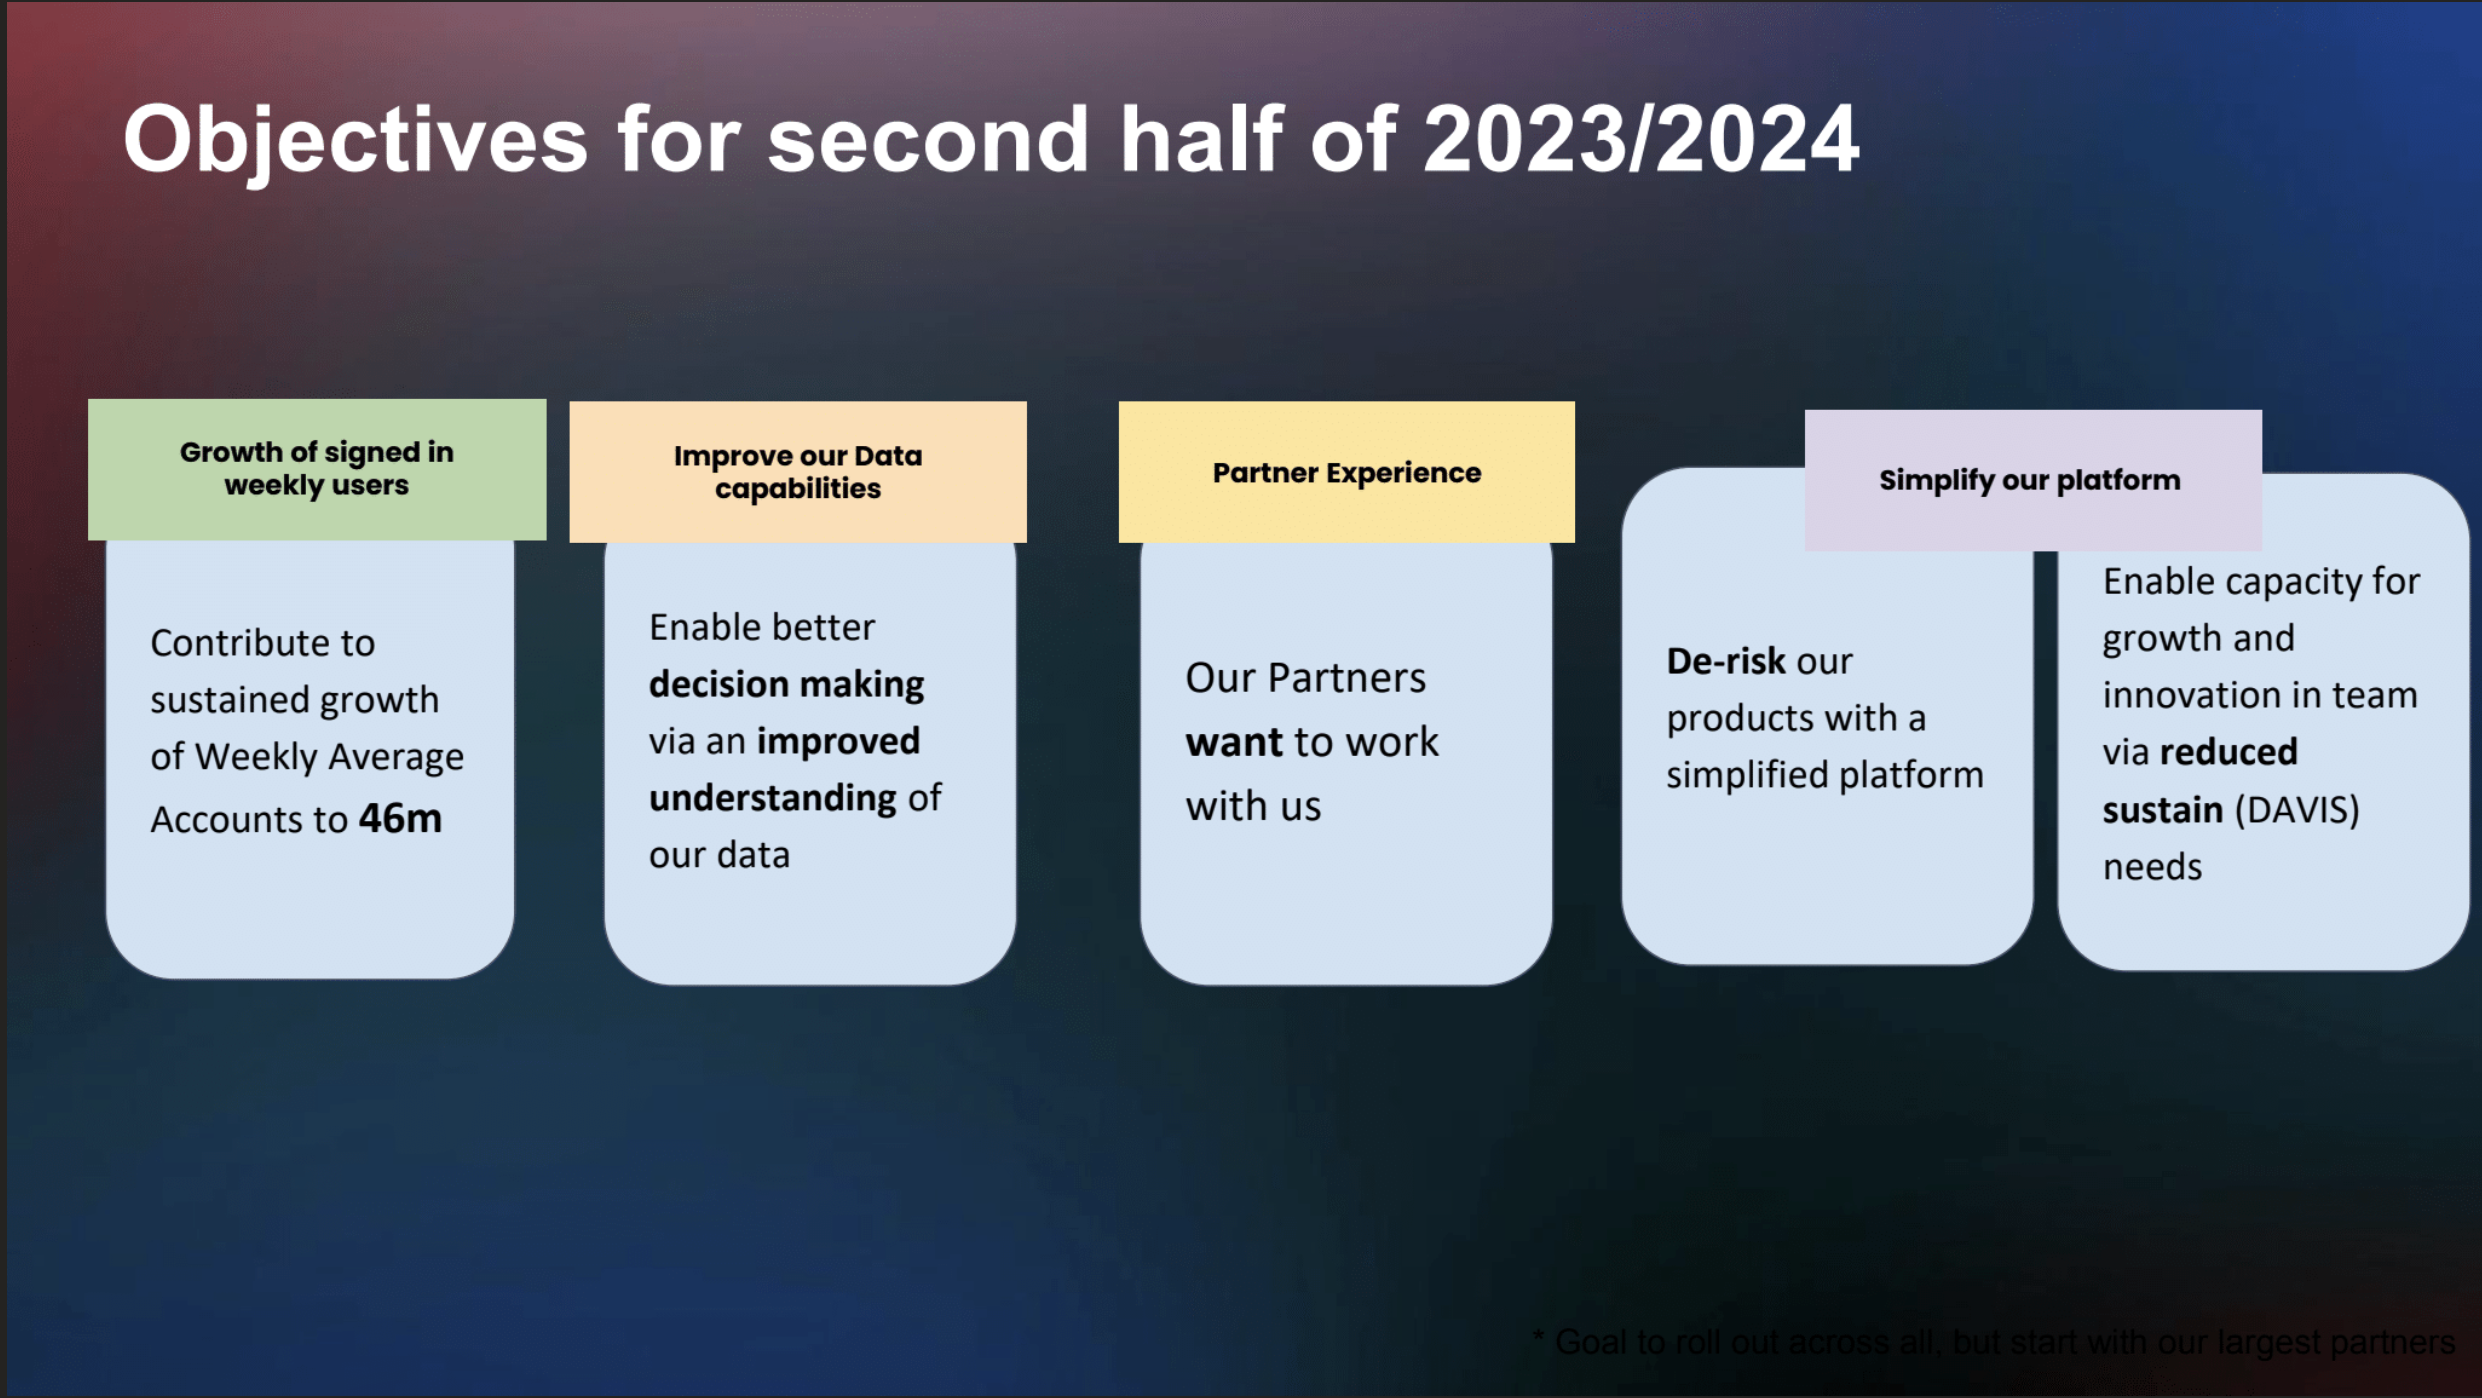
\includegraphics[width=12cm]{assets/appendix/partnershipsObjectives.png}
      \caption{Image taken from a presentation given at a partnerships context setting event (BBC Partnerships, 2023).}
      \label{fig:partnershipsObjectives}
    \end{figure}

  \newpage
  \subsection{Appendix B - Full schedules design including future external notification work}
    \label{sec:AppendixB}
    \begin{figure}[H]
      \centering
      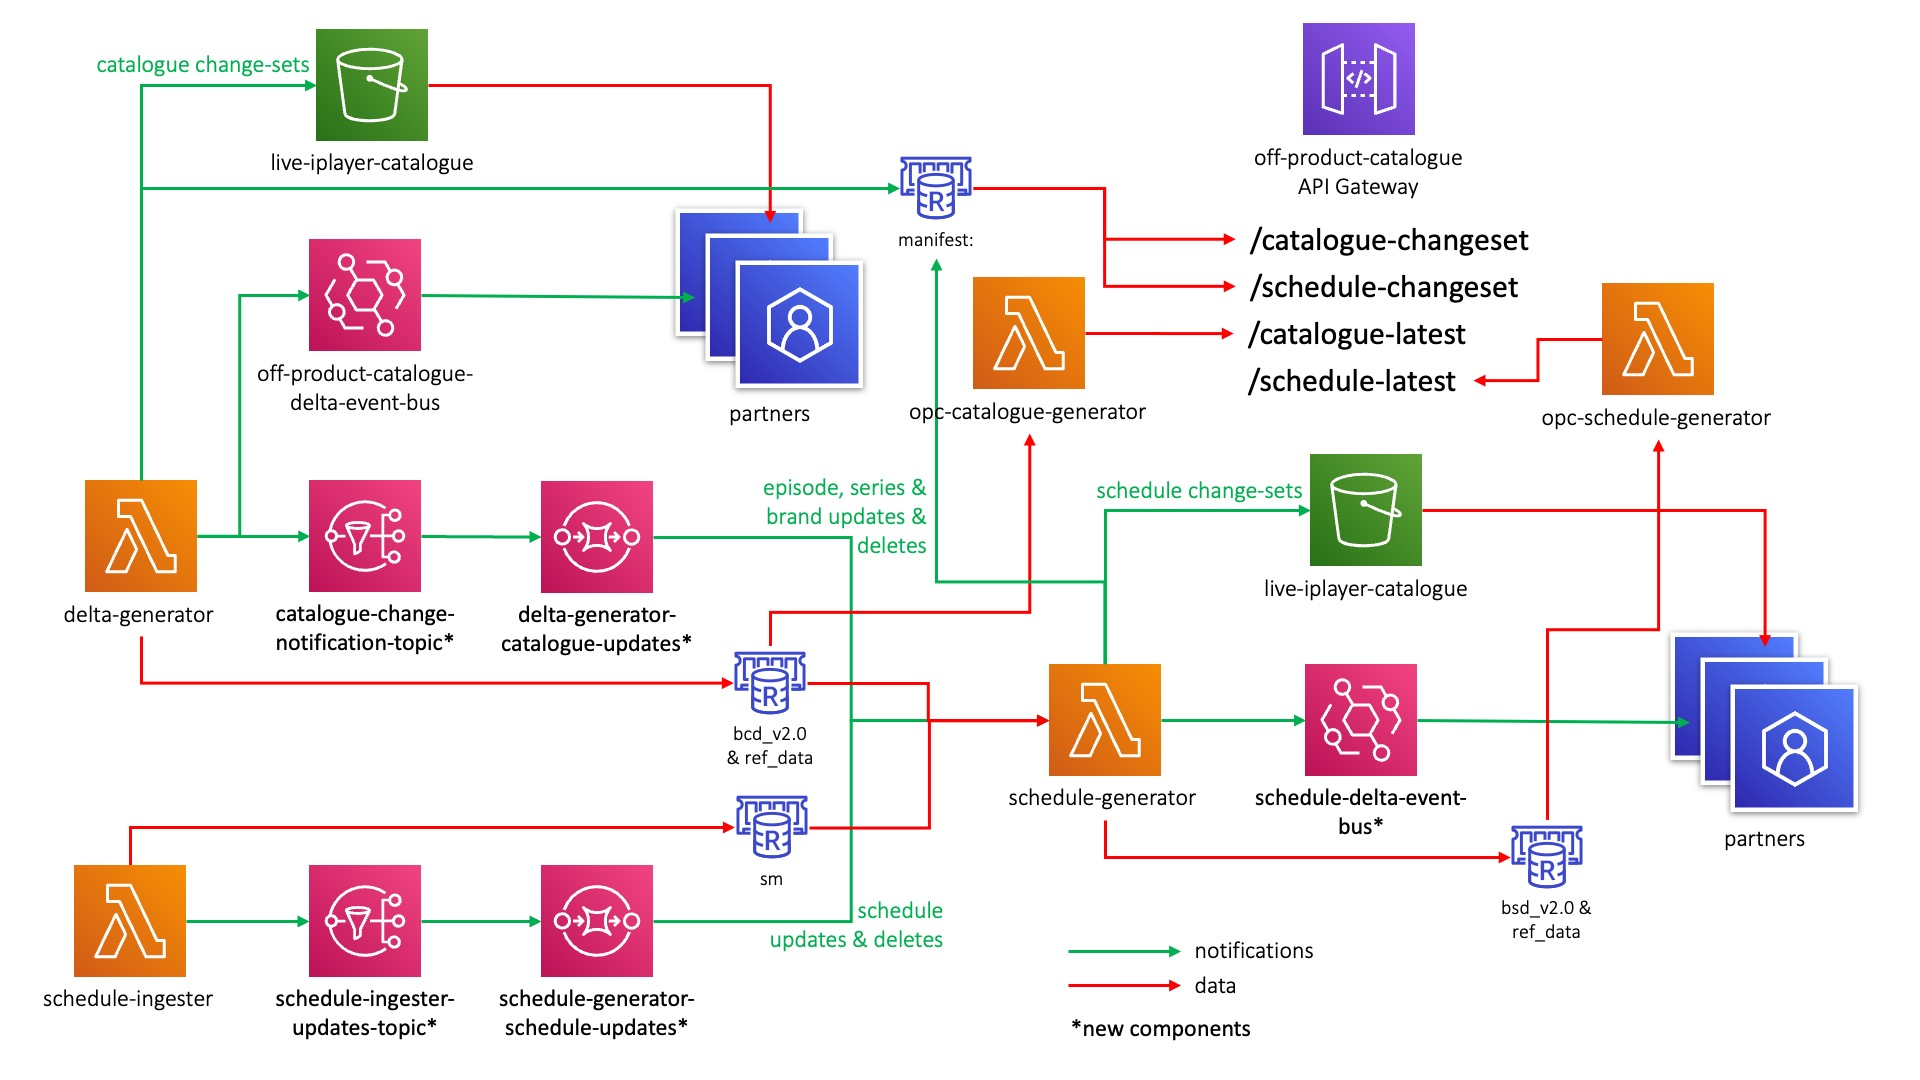
\includegraphics[width=12cm]{assets/appendix/initialDesign.jpg}
      \caption{Full diagram of design for schedules pipeline, including future notifications to partners work (Lloyd, 2023).}
      \label{fig:fullSpikeDesign}
    \end{figure}


  \newpage
  \subsection{Appendix C - Initial flow diagrams for how events would be processed}
    \label{sec:AppendixC}
    \begin{figure}[H]
      \centering
      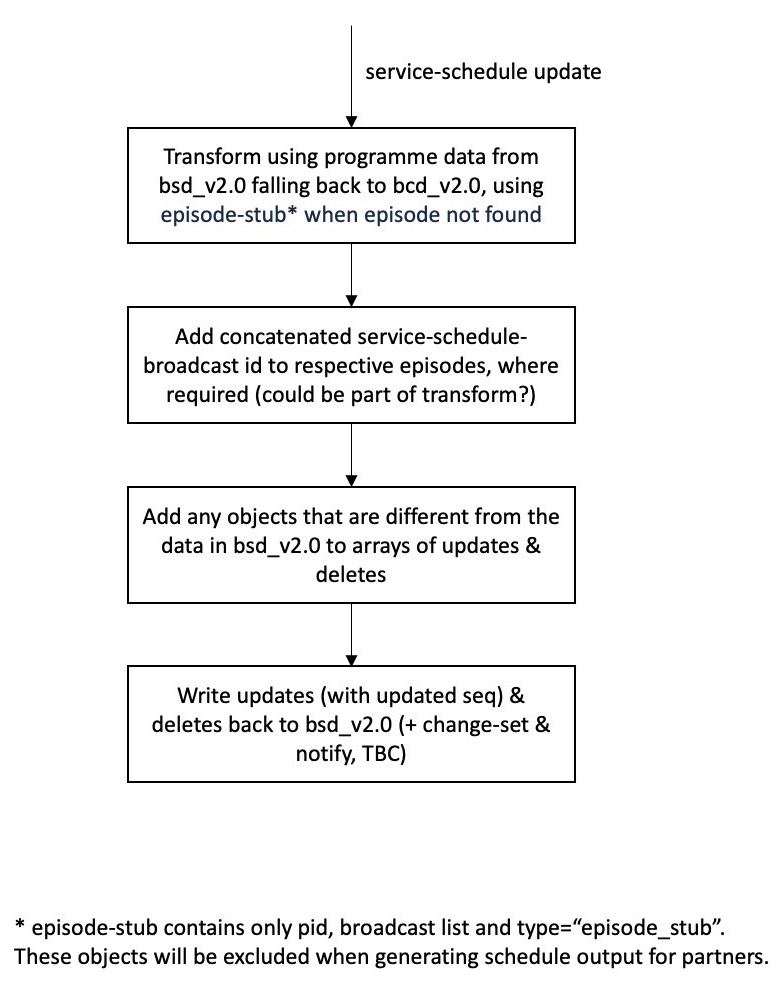
\includegraphics[width=6cm]{assets/initialDesign/scheduleUpdate.jpeg}
      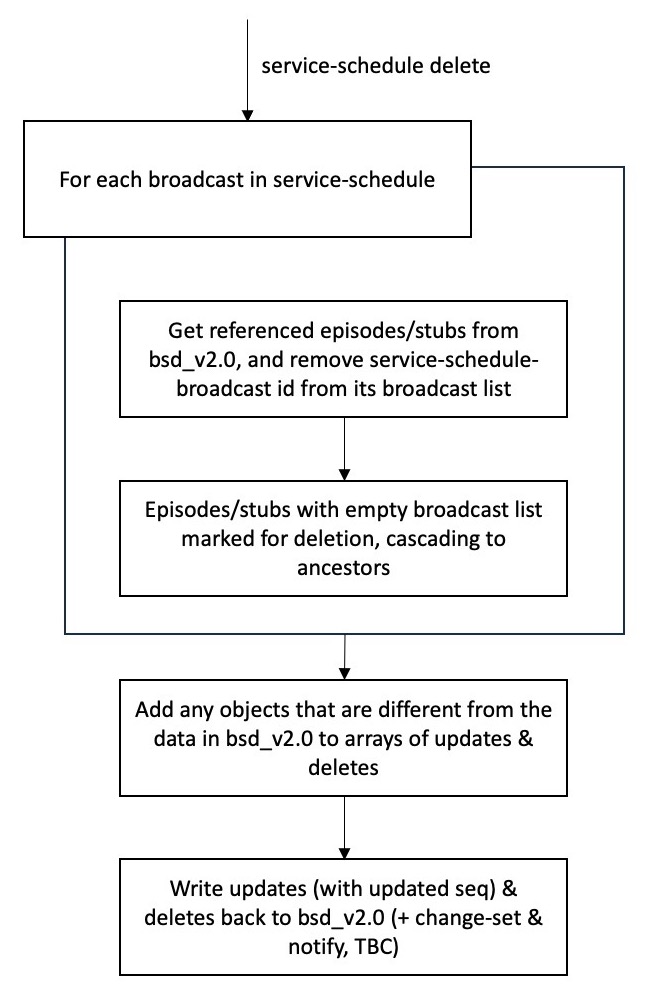
\includegraphics[width=6cm]{assets/initialDesign/scheduleDelete.jpeg}
      \caption{Flow diagrams for schedule events (Lloyd, 2023).}
      \label{fig:initialDesignSchedules}
    \end{figure}


    \begin{figure}[H]
      \centering
      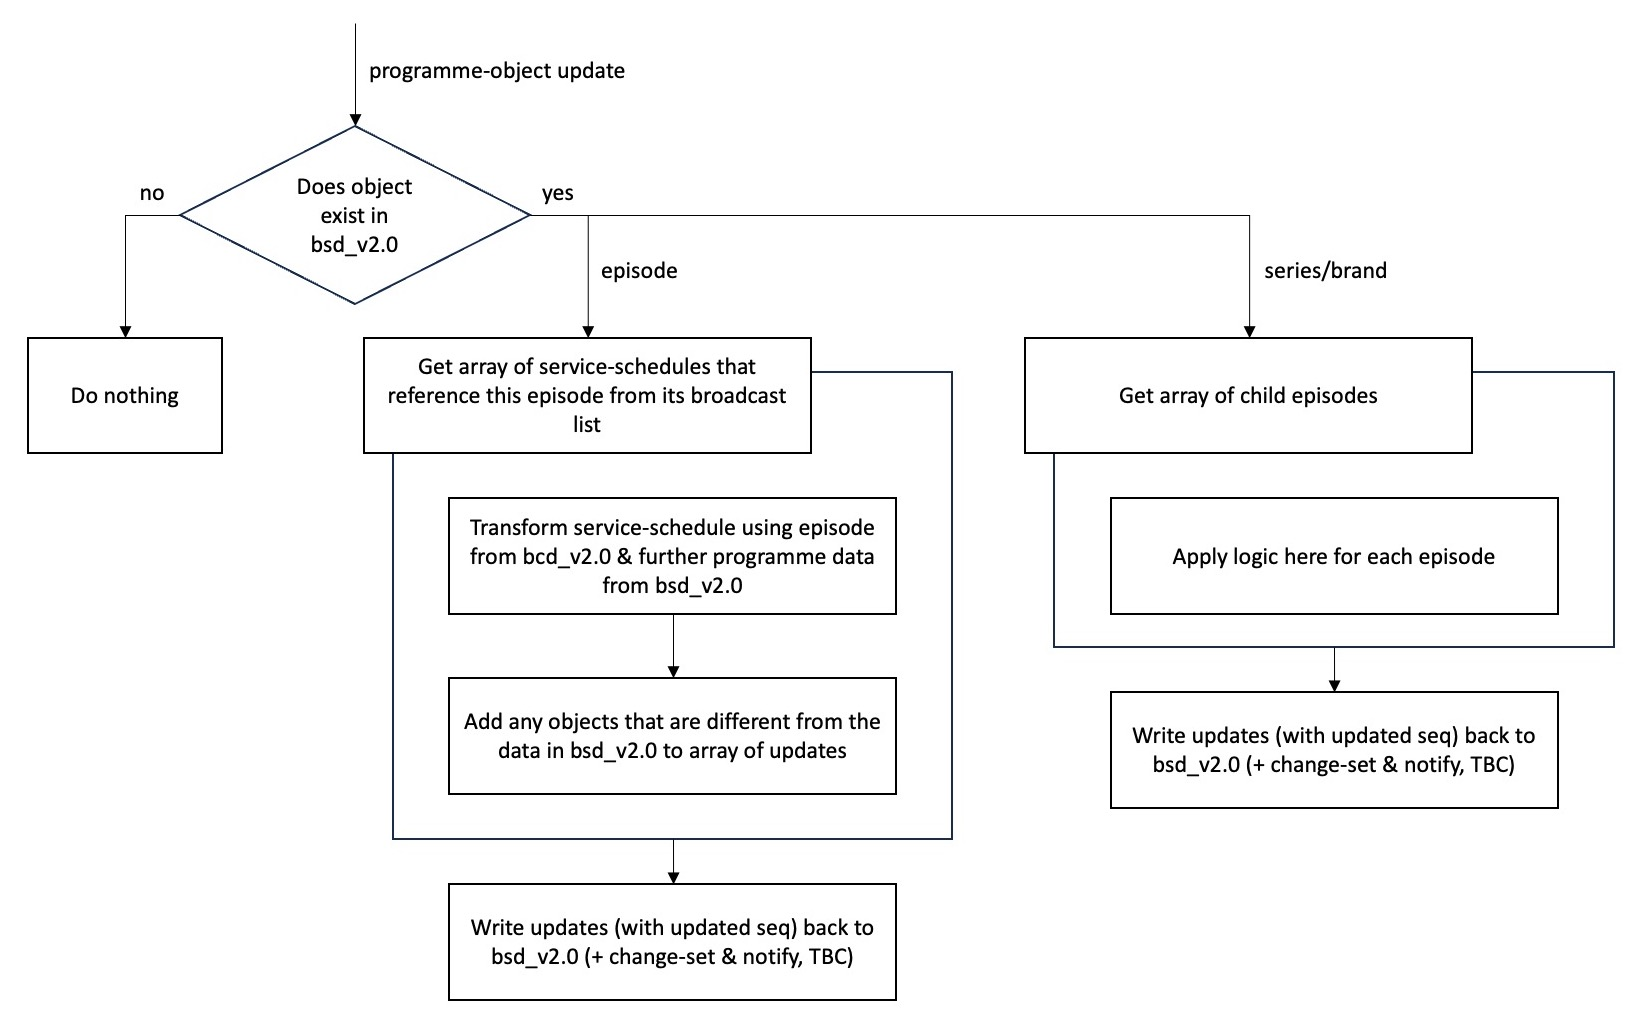
\includegraphics[width=12cm]{assets/initialDesign/programmeUpdate.jpg}
      \caption{Flow diagram for catalogue/programme events (Lloyd, 2023).}
      \label{fig:initialDesignProgrammes}
    \end{figure}

  
  \newpage
  \subsection{Appendix D - Full ways of working diagram}
    \label{sec:AppendixD}
    \begin{figure}[H]
      \centering
      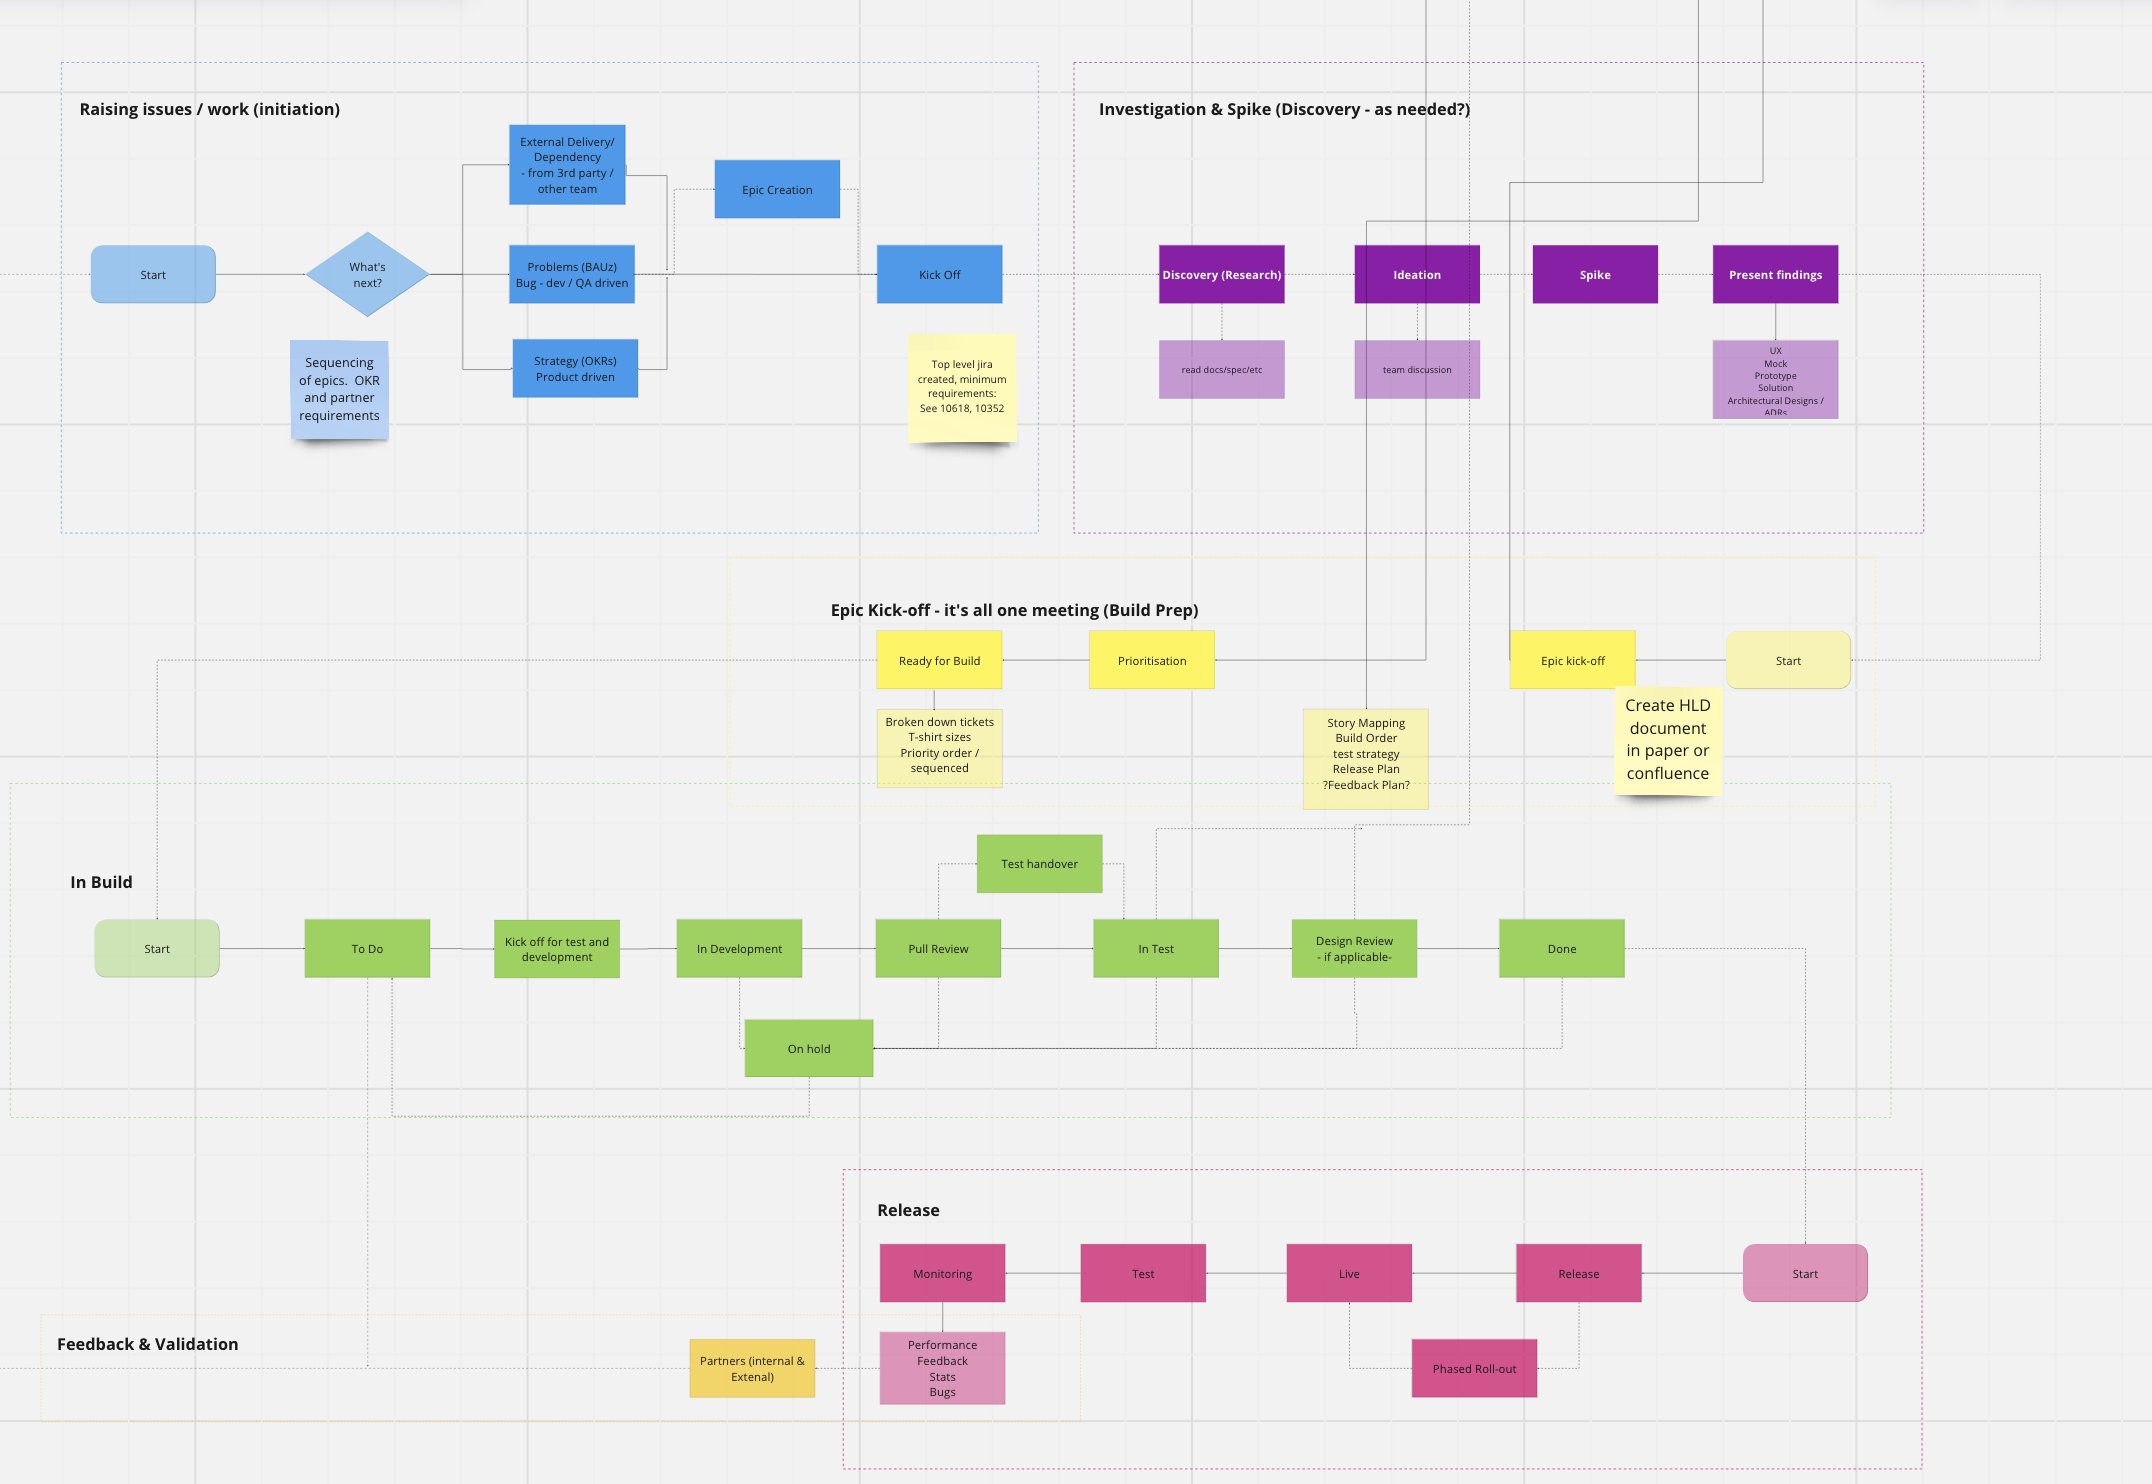
\includegraphics[width=12cm]{assets/workflow/fullWorkflow.png}
      \caption{Full ways of working flow diagram used by SpaceChimp.}
      \label{fig:fullWorkflow}
    \end{figure}


  \newpage
  \subsection{Appendix E - Full software spike document}
    \label{sec:AppendixE}
    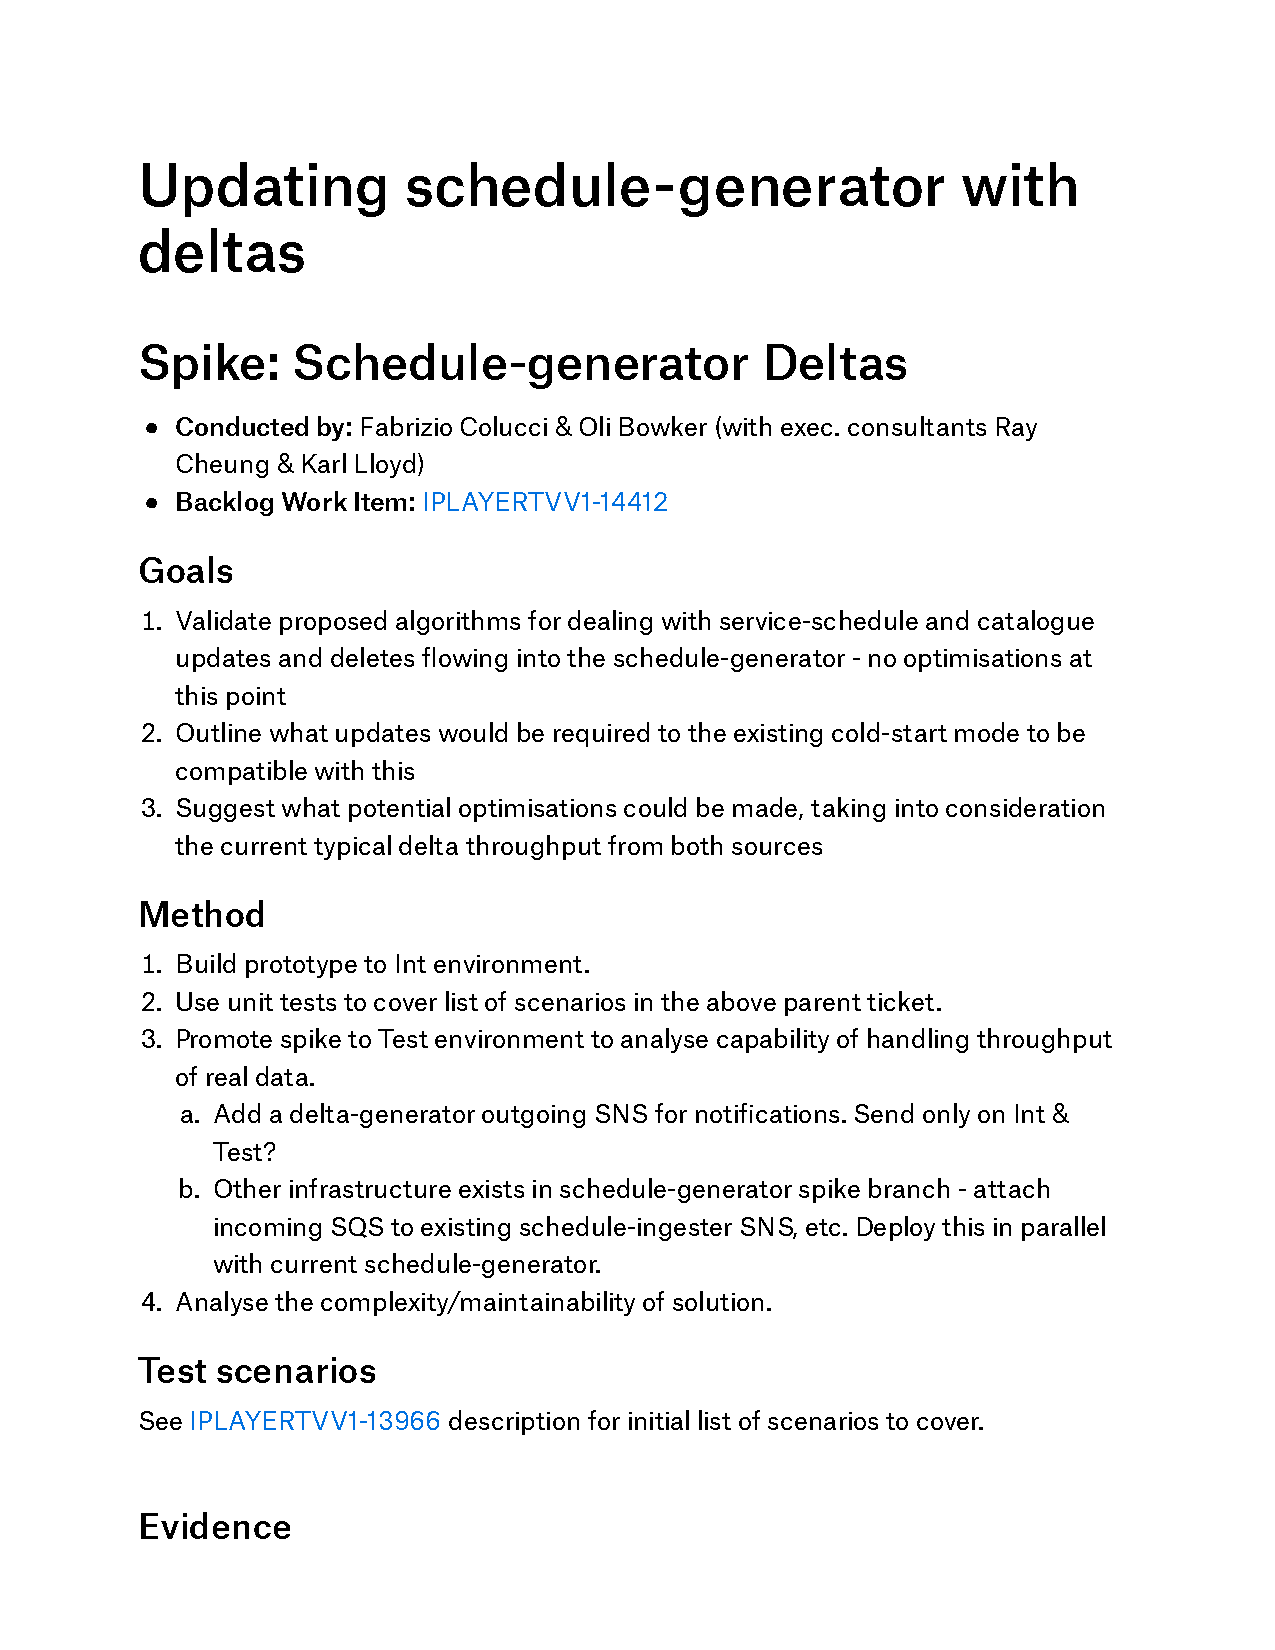
\includepdf[pages=-,scale=.6]{documents/spike.pdf}

  
  \newpage
  \subsection{Appendix !TODO! - Competency Mappings and Links}
    \begin{longtable}{|p{2.5cm}|p{10cm}|p{1.5cm}|}
      \hline
      \textbf{Competency} & \textbf{Description} & \textbf{Page} \\ \hline
      B1                  & Identify, document, review, and design complex IT-enabled business
                            processes that define a set of activities that will accomplish specific
                            organisational goals and that provide a systematic approach to im-
                            proving those processes. & \hyperref[sec:cicd]{Page X} \\ \hline

      P3                  & Professionally present digital-and-technology-solution-specialism plans
                            and solutions in a well- structured business report. & \hyperref[sec:cicd]{Page X} \\ \hline

      P4                  & Demonstrate self-direction and originality in solving problems, and
                            act autonomously in planning and implementing digital-and-technology-
                            solution-specialist tasks at a professional level. & \hyperref[sec:cicd]{Page X} \\ \hline

      P5                  & Be competent at negotiating and closing techniques in a range of
                            interactions and engagements, both with senior internal stakeholders
                            and external stakeholders. & \hyperref[sec:cicd]{Page X} \\ \hline

      SE-S01              & Architect, build, and support leading-edge concurrent-software plat-
                            forms that are performant to industry standards and that deliver
                            responsive solutions with good test coverage. & \hyperref[sec:cicd]{Page X} \\ \hline

      SE-S02              & Drive the technology-decision-making and development process for
                            projects of varying scales, considering current technologies including
                            DevOps and Cloud Computing, and evaluate different technology-
                            design and implementation options, making reasoned proposals and
                            recommendations. & \hyperref[sec:cicd]{Page X} \\ \hline

      SE-S03              & Develop and deliver distributed or semi-complex software solutions
                            that are scalable, and that deliver innovative user experiences and
                            journeys that encompass cross-functional teams, platforms, and technologies. & \hyperref[sec:cicd]{Page X} \\ \hline

      SE-S04              & Update current software products, improving their efficiency and
                            functionality, and build new features to product specifications. & \hyperref[sec:cicd]{Page X} \\ \hline

      SE-S05              & Accomplish planned software-development tasks that deliver the expected
                            features within specified time constraints, security, and quality requirements. & \hyperref[sec:cicd]{Page X} \\ \hline

      SE-S06              & Be accountable for the quality of deliverables from one or more
                            software-development teams (source code quality, automated testing,
                            design quality, documentation, etc.), and following company-
                            standard processes (code reviews, unit testing, source code management, etc.)  & \hyperref[sec:cicd]{Page X} \\ \hline

      SE-K02              & The various inputs, statements of requirements, security considerations
                            and constraints that guide solution architecture and the development
                            of logical and physical systems' designs. & \hyperref[sec:cicd]{Page X} \\ \hline

      SE-K03              & The methodologies designed to help create approaches for organizing
                            the software-engineering process, the activities that need to be
                            undertaken at different stages in the life-cycle, and techniques for
                            managing risks in delivering software solutions. & \hyperref[sec:cicd]{Page X} \\ \hline

      SE-K04              & The approaches used to modularise the internal structure of an
                            application, and to describe the structure and behaviour of applications
                            used in a business, with a focus on how they interact with each other
                            and with business users. & \hyperref[sec:cicd]{Page X} \\ \hline

      SE-K05              & How to design, develop, and deploy software solutions that are secure
                            and effective in delivering the requirements of stakeholders, and
                            the factors that affect the design of a successful code. & \hyperref[sec:cicd]{Page X} \\ \hline

      SE-K06              & The range of metrics which might be used to evaluate a delivered
                            software product. & \hyperref[sec:cicd]{Page X} \\ \hline

      
    \end{longtable}